\documentclass{book}
\usepackage[allcolors=true]{hyperref}
\usepackage{graphicx}
\usepackage{amsmath,amsfonts,amsthm,amssymb}

\newcommand\bg[2]{
\begin{center}
\fcolorbox{white}{BGgris}{\parbox{.9\linewidth}{\begin{large} \textit{#1} \end{large} \\
#2 }}
\end{center}}

\begin{document}
\chapter{De Planck à l'équation de Schrödinger}\label{chap:chap2}

\section{Dualité onde-corpuscule de la lumière}
La lumière a toujours été dans l'histoire une source d'interrogation. Elle nous sert à voir. Mais on peut aussi en étudier la nature. Corpuscule ? Ondulatoire ? Les deux hypothèses se combattaient au XVIIè siècle, avec Christophe Huygens qui défendait une théorie ondulatoire et Isaac Newton qui défendait une théorie corpusculaire. 

Au XIXè siècle, des expériences de diffraction (phénomène purement ondulatoire) menées par Thomas Young et Augustin Fresnel ont permis d'affirmer que la lumière possédait des propriétés ondulatoires. Newton part donc avec un point en moins. Un siècle plus tard, Einstein émet une théorie corpusculaire de la lumière, en s'inspirant des travaux de Planck. 

Max Planck voulait expliquer le rayonnement des corps noirs (enceinte macroscopique qui absorbe entièrement tout rayonnement incident, à l'équilibre thermodynamique entre la matière qui le constitue et son propre rayonnement). De son étude est ressorti un paramètre qui a les dimensions d'une énergie fois un temps (unités : $\mathrm{Js}$), appelé \textit{constante de Planck}. Ce paramètre qu'on note $h$ permet de décrire les propriétés du   rayonnement d'un corps noir, par exemple son spectre et sa densité d'énergie en fonction de la température (toujours, voir PHYS-F201). Le résultat obtenu par Planck n'était cependant pas en accord avec la mécanique classique. De son côté, Albert Einstein propose une théorie corpusculaire de la lumière, qui  en utilisant cette  constante $h$ décrit l'effet photoélectrique.
Ceci souligne l'importance de $h$ car le corps noir et le métal n'ont \textit{a priori} rien en commun. La constante de Planck est donc une des \textit{constantes fondamentales de l'Univers}:
$$h \approx 6.6 \times 10^{-34} \; \mathrm{Js}$$
%Le caractère fondamental de la constante de Planck lui procure également un autre surnom : le \textit{quantum d'action}.

{\it Remarque. Depuis le 20 mai 2019,  la 
valeur numérique de la constante de Planck, h, 
est choisie égale à 
6,626 070 15$ \times 10^{-34}\; \mathrm{Js}$, 
unité égale à $\mathrm{kg\; m^2\; s^{-1}}$. 
La seconde est définie en fixant la fréquence de la transition hyperfine de l’état fondamental de l’atome de césium 133 non perturbé comme égale à 9 192 631 770 Hz. 
Et la vitesse de  la vitesse de la lumière dans le vide, c, est fixée comme ayant une valeur numérique égale à 299 792 458 m/s. 
Par conséquent l'unité de masse, le kg, est déterminée en fonction de la définition de la seconde, de la vitesse de la lumière, et de la constante de Planck.}

\subsubsection{Effet photoélectrique}
En bombardant une plaque métallique de lumière de longueur d'onde $\lambda$ (maintenant qu'on sait que la lumière est une onde), on remarque qu'au-delà d'une certaine fréquence seuil $\nu_0$ ($\lambda$ et $\nu$ sont liées par $\lambda = c/\nu$), des électrons sont émis avec une énergie qui augmente linéairement avec la fréquence, avec une pente de $h$, et dont l'expression de son énergie cinétique $T$ est donnée par :

$$ T = h\nu - W$$
où $W = h \nu_0 \equiv$ travail d'extraction, autrement dit, c'est le travail que doit fournir l'électron pour s'extraire de la plaque métallique. L'interprétation est que chaque particule de lumière a une énergie $h \nu$.

\subsubsection{Les particules de lumière}
Einstein est amené à établir une relation entre la longueur d'onde de la lumière et une impulsion (à travers le nombre d'onde, ou plus précisément, le vecteur d'onde $\vec{k}$).
En effet, nous savons par le cours de relativité et électromagnétisme que l'énergie totale d'une particule est donnée par $E = m \gamma c^2$, tandis que l'impulsion vaut $\vec{p} = m \gamma \vec{v}$. Ainsi, nous avons la relation $\vec{p} = \frac{E}{c^2} \vec{v}$. 
Or si l'on considère bien la lumière comme une particule, nous pouvons exploiter ces relations. Sa vitesse étant de plus constante, de norme $c$, nous en déduisons que : 
\begin{align*}
  p &= \frac{E}{c^2} c = \frac{E}{c} = \frac{1}{c} \hbar \omega \\
  &= \hbar k 
\end{align*}
où nous avons employé la relation de dispersion pour la lumière $\omega = kc$. \\
Le fait que $E = pc$ nous donne, par $E^2 = m^2 c^4 + c^2 p^2$, que la particule qui décrit la lumière est de masse nulle. \\
En résumé, nous avons donc ces deux relations très importantes qui relient la lumière, une onde, à un caractère corpusculaire ; 
\begin{align}
\label{Quantification energie et impulsion}
\left\{ \begin{array}{l}
E \equiv \hbar \omega \quad \text{\small (quantification de l'énergie : lien énergie - fréquence}) \\
\vec{p} \equiv \hbar \vec{k}  \quad \text{\small (lien longueur d'onde-impulsion)}
\end{array} \right.
\end{align}

L'introduction d'une particule de lumière, portant le nom de \textbf{photon} est critiquée et nécessite  d'être démontrée. C'est ce qu'a fait Arthur Compton expérimentalement. Il a démontré que lors d'une interaction (une collision) photon-électron, l'impulsion et l'énergie de l'ensemble photon + électron étaient conservées, tout comme une particule classique. Le photon est donc bien une particule. Et c'est aussi une onde (\textit{cf.} franges de Young). 
\begin{center}
\begin{large}
\textit{La lumière se comporte donc à la fois comme une onde \underline{et} comme une particule.}
\end{large}
\end{center}

\subsection{Observation de la dualité onde-particule de la lumière}
On reprend l'expérience des fentes de Young et cette fois-ci en lumière atténuée, pour voir la figure d'interférence se construire progressivement. On alors les impacts un par un, \textbf{photon par photon} mais à long terme on voit se dessiner une figure d'interférence, voir Figure \ref{TwoSlit}. La lumière est à la fois constitué de particules (détectées une par une par la caméra), et une onde qui passe par les deux fentes à la fois. On parle de {\bf dualité onde-particule}.

\begin{figure}
\includegraphics[width=1.0\linewidth]{images/TwoSlitPhoton_2}
\caption{Expérience (moderne) de Young avec un faisceau laser atténué. Chaque image enregistre quelques photons (pixels vert sur l'image "1 frame"). En accumulant les images, on voit apparaitre les franges d'interférence. En bas, schéma de l'expérience. Source "The wave-particle duality of light: A demonstration experiment",
  T. L. Dimitrova and Antoine Weis, American Journal of Physics 76, 137-142 (2008).
}
\label{TwoSlit}
\end{figure}





Einstein a ainsi développé et cru en une théorie qui allait à l'encontre de ce qui avait été imaginé et prouvé par l'expérience depuis le siècle précédant. Et ce malgré la splendide explication théorique de l'électromagnétisme par Maxwell.

\section{Dualité onde-corpuscule de la matière}
L'aspect corpusculaire de la matière n'a pas besoin d'être introduit. En revanche, son aspect ondulatoire nourrit les interrogations rien qu'à l'usage de l'expression. C'est Louis de Broglie le véritable héros derrière cette hypothèse.

\subsection{Hypothèse de de Broglie}

Dans la section précédente, nous avons argumenté qu'un rayonnement lumineux de fréquence $\nu$ est constitué de corpuscules porteur d'énergie $E = h \nu$. 

A la même époque, les spectres d'émission et d'absorption des atomes (notamment l'hydrogène) étaient étudiés, et la quantification de l'énergie de ces atomes permettait d'expliquer le fait que l'on observait un spectre de raies fines distinctes. 

En effet, en supposant qu'un atome fasse une transition entre un état d'énergie $E_i$ et $E_j$, un photon d'énergie 
$$E_{ij} =  |E_i - E_j|= h\nu_{ij} $$
ou nous avons utilisé la relation énergie-fréquence pour le photon pour lier 
l'énergie de la transition à la fréquence de la lumière émise (ou absorbée, suviant le processus).



La mécanique classique ne permettant pas d'expliquer ce phénomène.
Bohr a construit son célèbre modèle qui donne une base pour la quantification de l'énergie des atomes. Mais comment justifier le modèle de Bohr?

Louis de Broglie a alors émis l'hypothèse 
%\wrap{15}{r}{0.4}{\centering \vspace{-0.5cm}
\begin{figure}
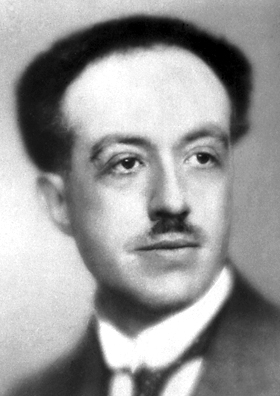
\includegraphics[width=0.3\linewidth]{images/Louis_de_Broglie}
\caption{Louis de Broglie. Il obtint le prix Nobel en 1929 à 37 ans pour la découverte de la nature ondulatoire de l'électron.}
\end{figure}
%}
que \textbf{tous les corpuscules matériels ont également un aspect ondulatoire}, et que les aspects corpuscule et ondulatoire sont reliés par la formule 
\begin{equation} \label{eq:debroglie}
\boxed{
 \lambda = \frac{h}{p} \quad \text{ \textit{(Relation de de Broglie).}}} 
\end{equation}
A une particule d'impulsion $p$, on associe donc une longueur d'onde $\lambda$.

Par analogie avec la relation pour les photons \eqref{Quantification energie et impulsion}, on peut postuler que pour une particule matérielle, on peut associer une fréquence à la particule et une
\begin{equation} \label{eq:debroglie}
\boxed{
\left\{ \begin{array}{ll}
E &= \hbar \omega \\
\vec p &= \hbar \vec k
\end{array} \right. } 
\end{equation}


Notons que l'hypothèse de de Broglie a été vérifiée ultérieuremnet en montrant que des électrons montrent des figures d'interférence. Et plus récemment en montrant que des atomes, et même des molécules complexes, peuvent aussi montrer des figures d'interférence.



\subsection{Vers l'équation de Schrödinger}

Sur base des relations de de Broglie, il serait utile de décrire mathmatiquement une particule en prenant en compte son charactère ondulatoire. 
C'est ce qu'entreprends Schrödinger, qui veut écire une équation d'onde pour les particules matérielles.

Nous allons maintenant montrer comment arriver à l'équation de Schrödinger, autrement dit, comment  établir une relation qui décrit une particule quantique de manière ondulatoire. 


Pour y arriver, faisons un pas en arrière, et considérons l'équation d'onde la plus simple à 3 dimensions
$$\left(\dfrac{1}{c^2} \partial_t ^2 - \Delta \right) \vec A = 0\ .$$
Une solution possible de cette équation est l'onde place, c'est-à-dire une fonction de la forme : $$
A(\vec{x}, t) = A_0 \; e^{-i(\omega t - \vec k \cdot \vec x)} \; .$$
Par conséquent, si nous supposons $A(\vec r, t)$ connu, nous pouvons retrouver la fréquence et le nombre d'onde en effectuant des dérivées:
\begin{eqnarray}
\omega &=&\dfrac{i}{A} \partial_t A \nonumber\\
\omega^2 &=&-\dfrac{1}{A} \partial_t^2 A \nonumber\\
  \vec k &=& -\dfrac{i}{A} \vec \nabla A \nonumber\\
  k^2 &=& -\dfrac{1}{A} \Delta A\label{eq:Ader}
\end{eqnarray}

Supposons maintenant que nous cherchons à écrire une équation d'onde pour laquelle nous postulons une relation $\omega = f(k)$ liant la fréquence au nombre d'onde. En utilisant les relations \eqref{eq:Ader}, ou des relations similaires, nous pouvons transformer notre relation $\omega = f(k)$ en une équation aux dérivées partielles pour $A$. (Cette démarche ne donne pas une équation unique. Par exemple on pourrait utiliser $\omega^2 = \left(\dfrac{i}{A} \partial_t A  \right)^2$ plustot que $\omega^2 =-\dfrac{1}{A} \partial_t^2 A$. On essayera néanmoins d'obtenir une équation linéaire).

Appliquons cette approche en utilisant les relations de de Broglie.

(1) {\bf Particule libre relativiste} décrite par
$$E^2 = m^2 c^4 + p^2 c^2\ .$$
Les relations de de Broglie permettent de tirer de cette relation une relation entre la fréquence et le nombre d'onde de la particule
$$\hbar^2 \omega^2 = m^2 c^4 + \hbar^2 k^2 c^2\ .$$
Il est habituel dans ce cas de noter l'onde associée par $\phi$. En utilisant \eqref{eq:Ader} on obtient 
 l'\textbf{équation de Klein-Gordon}.
\begin{equation} 
\boxed{\text{Équation de Klein-Gordon} : \quad -\hbar ^2 \partial_t ^2 \phi + c^2 \hbar ^2 \Delta \phi - c^4 m^2 \phi = 0}
\label{Eq:KG}
\end{equation}
Cette équation est d'ordre  2 en le temps, ce qui rends son interprétation compliquée. Elle constitue la base pour l'étude de la mécanique quantique relativiste.

(2) {\bf Particule non relativiste dans un potentiel} décrite par
$$E = \dfrac{p^2}{2m} + V(\vec r, t)\ .$$
Les relations de de Broglie permettent de tirer de cette relation une relation entre la fréquence et le nombre d'onde de la particule
$$\hbar \omega =  \dfrac{\hbar^2 k^2}{2m}  + V(\vec r, t)\ .$$
Dans ce cas il est habituel de noter l'onde associée par $\psi(\vec r, t)$. 
En substituant \eqref{eq:Ader} on obtient  
\begin{equation} 
i\hbar \dfrac{1}{\psi} \dfrac{\partial}{\partial t} \psi = - \dfrac{1}{\psi}  \dfrac{\hbar ^2}{2m} \Delta \psi + V(\vec r, t)\ .
\end{equation}
En multipliant par $\psi$ on obtient la forme traditionelle de 
\textbf{ l'équation de Schrödinger} :
\begin{equation} 
\boxed{\text{Équation de Schrödinger} : \quad
i\hbar \dfrac{\partial}{\partial t} \psi = -\dfrac{\hbar ^2}{2m} \Delta \psi + V(\vec r, t) \psi}
\label{Eq:S}
\end{equation}

Il faut noter que la procédure pour arriver aux équations \eqref{Eq:KG} et \eqref{Eq:S} n'est pas unique. Un choix important a été fait, c'est de formuler l'équation d'onde comme une équation linéaire (C'est à dire que si $\psi_1$ et $\psi_2$ sont solutions, alors $a \psi_1 + b \psi_2$ est aussi solution). 

Que l'équation obtenue soit utile et relevant pour la physique n'est pas garanti. Schrödinger a immédiatement testé son équation dans le cas de l'atome d'Hydrogène $V(\vec r, t) = \frac{k q^2}{r}$. Le fait qu'il a trouvé les mêmes niveaux d'énergie que dans le modèle de Bohr indique qu'il est sur la bonne voie. Son équation, et ses extensions, servira de base pour décrire les phénomènes quantiques.

Notons qu'en même temps que Schrödinger, Heisenberg trouve également une manière de décrire mathématiquement les phénomènes quantiques. L'approche de Heisenberg consiste à remplacer les grandeurs classiques $x$ et $p$ par des opérateurs. Il applique sa méthode à l'oscillateur harmonique. Son approche est plus difficile à utiliser que celle de Schrödinger, mais néanmoins dans certains cas fort utile. Schrödinger montre peu après que les deux approches sont équivalentes. Dans ce cours nous utiliserons exclusivement l'approche de Schrödinger.





\end{document}
